\section{Results}\label{sec:result}
Figure \ref{fig:result} shows our measured $\sigma_{\mathrm{ABS}}$ and $\sigma_{\mathrm{CX}}$ with statistical and systematic error bars as a function of pion momentum, compared with the results from previous experiments \cite{Bellotti1973,Ashery2,Bellotti1973_2,Jones}. Our result are in agreement with previous experiments. As summarized in Table \ref{table:systematics}, the total error is $\sim$9.5\% for $\sigma_{\mathrm{ABS}}$ and $\sim$18\% for $\sigma_{\mathrm{CX}}$, except fot the $p_{\pi}$ = 216.6 MeV$/c$ data set.

\begin{figure}[h]
\begin{center}
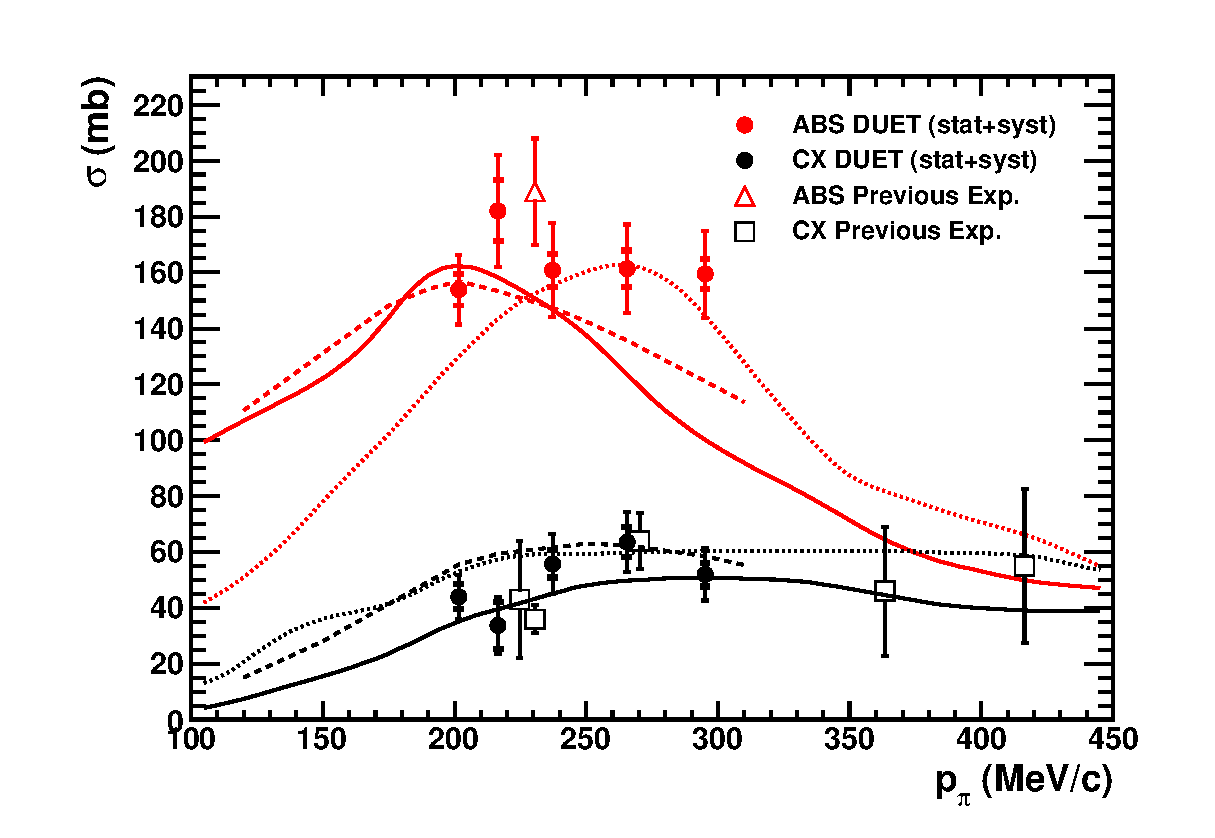
\includegraphics[width=86mm]{figures/duet_result_for_sep_paper.eps}
\caption{(Color online) DUET measurements of $\sigma_{\mathrm{ABS}}$ and $\sigma_{\mathrm{CX}}$ compared with previous measurements and ABS (red) and CX (black) model predictions from \textsc{Geant4} (solid line), \textsc{Fluka} (dashed line) and \textsc{Neut} (dotted line).}
\label{fig:result}
\end{center} 
\end{figure}

Figure \ref{fig:covariance} shows the fractional covariance matrix for the 5 $\sigma_{\mathrm{ABS}}$ and 5 $\sigma_{\mathrm{CX}}$ measured data points. The statistical uncertaitinties were included as an un-correlated, diagonal matrix. There are small positive correlations with the ABS and CX points, and some negative correlations across them, as is expected from the subtraction method used. This is the first time that a correlation matrix is published for pion inelastic cross sections. It is expected to provide additional insight to the proper modeling and tuning of hadron-nucleus inelastic interactions.

\begin{figure}[h]
\begin{center}
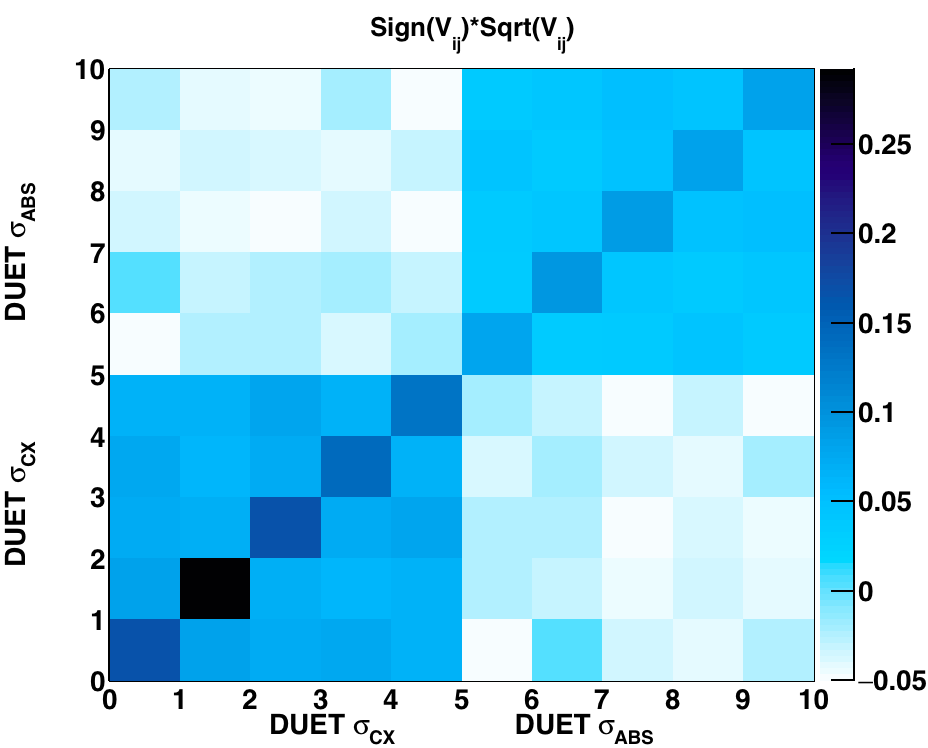
\includegraphics[width=80mm]{figures/duet_covariance_for_research_evaluation_png.png}
\caption{Fractional covariance matrix for the DUET measurements of $\sigma_{\mathrm{ABS}}$ and $\sigma_{\mathrm{CX}}$. }
\label{fig:covariance}
\end{center} 
\end{figure}

\section{Summary}
To summarize, we obtained the separate ABS and CX cross sections of positive pions in carbon nuclei at five incident momenta between 201.6 MeV$/c$ to 295.1 MeV$/c$. A covariance matrix for the 10 measured data points was produced. This result will be an important input to existing models such as \textsc{Geant4} or \textsc{NEUT} to constrain sub-GeV pion interactions.
